\documentclass{standalone}
\usepackage{tikz}
\usepackage{verbatim}
\usetikzlibrary{positioning}
\begin{document}
\pagestyle{empty}
  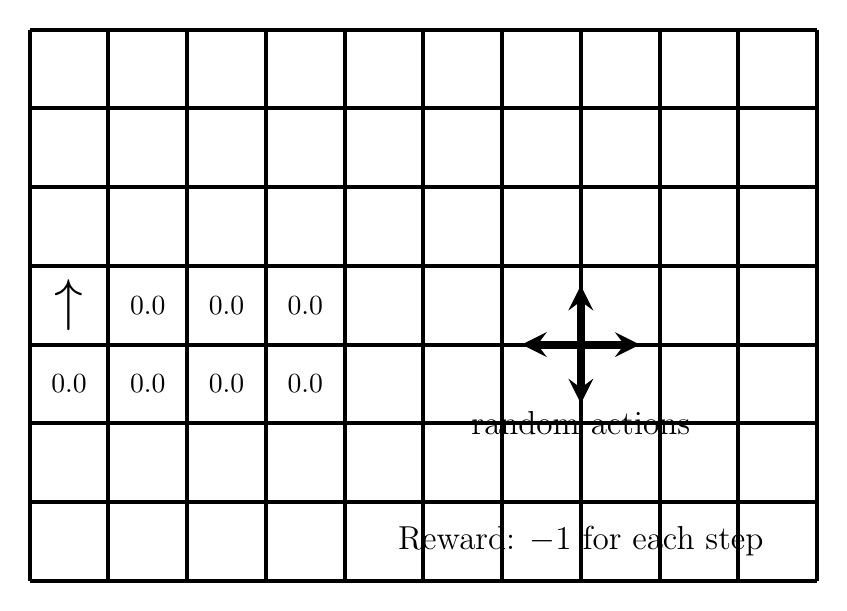
\begin{tikzpicture}
    \draw[stealth-stealth, line width=1 mm] (7.75, 3) -- (6.25, 3);
    \draw[stealth-stealth, line width=1 mm] (7, 2.25) -- (7, 3.75);
    \node at (7, 2) {\large random actions};
    \node at (7, 0.5) {\large Reward: $-1$ for each step};
    % Top row.
    \node at (0.5, 3.5) {\huge $\uparrow$};
    \node at (1.5, 3.5) {0.0};
    \node at (2.5, 3.5) {0.0};
    \node at (3.5, 3.5) {0.0};
    % Second frop top row.
    \node at (0.5, 2.5) {0.0};
    \node at (1.5, 2.5) {0.0};
    \node at (2.5, 2.5) {0.0};
    \node at (3.5, 2.5) {0.0};

    \draw[step=1.0,black, line width=0.5 mm] (0,0) grid (10, 7);
  \end{tikzpicture}
\end{document}